\begin{figure}[hbt!]
    \centering
    \caption{Estimated shares pocketed by landlords for different values of 
             the elasticity of wage income to the MW}
    \label{fig:cf_share_by_epsilon}

    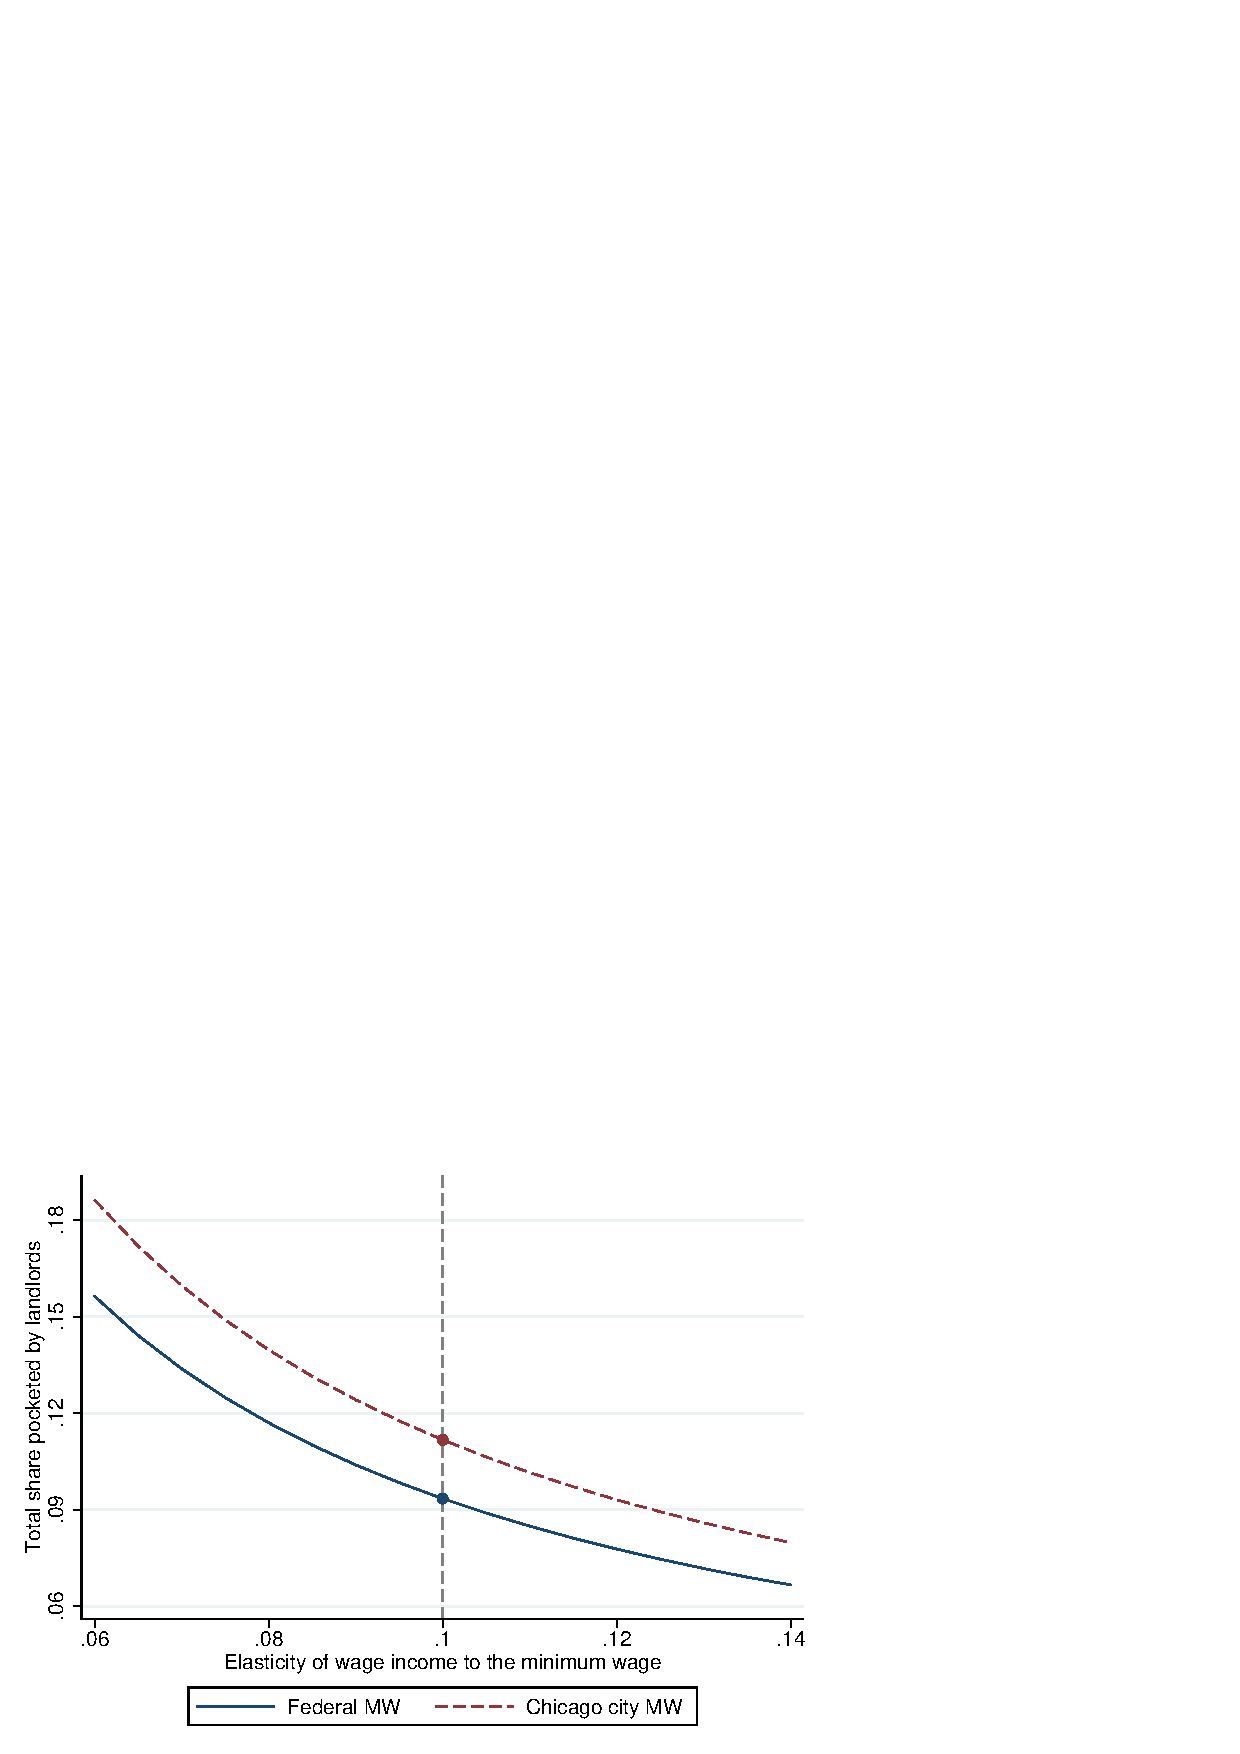
\includegraphics[width = .75\textwidth]{counterfactuals/output/incidence_by_epsilon}

    \begin{minipage}{.95\textwidth} \footnotesize
        \vspace{3mm}
        Notes:
        Data are from the MW panel described in section \ref{sec:data_mw_panel} 
        and from LODES.
        The figures show the estimated ZIP-code specific share of additional 
        income pocketed by landlords (``share pocketed'')
        under different counterfactual policies:
        an increase to \$9 in the federal MW in January 2020, and
        an increase from \$13 to \$14 in the Chicago City MW, 
        both holding constant other MW policies.
        The unit of observation is the ZIP code.
        To estimate it we follow the procedure described in Section 
        \ref{sec:counterfactual}, assuming the following parameter values: 
        $\beta = \betaCf$, $\gamma = \gammaCf$. 
        The x-axis shows a range of values for the elasticity of wage 
        income to the minimum wage $\varepsilon$.
        The line at $\epsilon=0.1$ corresponds to the estimates reported in
        Table \ref{tab:counterfactuals}.
    \end{minipage}
\end{figure}
